\documentclass[12pt,xcolor=dvipsnames,table,titlepage]{beamer}
\usetheme{CambridgeUS}
\usecolortheme{whale}
\setbeamercolor{block title}{use=structure,fg=white,bg=blue!75!black}  
\setbeamercolor{block body}{use=structure,fg=black,bg=blue!5!white}
\setbeamercolor{frametitle}{bg=Blue}
\usepackage{hyperref}   
\usepackage{url}
\hypersetup{urlcolor=red}
\renewcommand{\bibname}{References}
\usepackage{amsmath,amssymb}
\usepackage{mathtools}
\setbeamertemplate{bibliography item}{[\theenumiv]}
\usepackage{multicol}
\usepackage{multirow}
\usepackage{verbatim} 
\RequirePackage[singlelinecheck=off]{caption}
\usepackage{graphics}
\usepackage[utf8]{inputenc}
%\titlehead{
\includegraphics[width=33, height=25]{logo1.png}

\begin{document}
%Basic Information

\title{Sentiment Analysis in Twitter}
\author[]{ 
\includegraphics[width=35, height=28]{logo1.png} \\ \underline{Team Members}\\Rajarshi Sarkar (BE/1397/11) \\ Amit Kumar (BE/1513/11) \\~\\ \underline{Project Mentor}\\ Dr. Vijay Kumar Jha \\~\\ IT8020 Project\\Birla Institute of Technology, Mesra}
\date{\today}
}

%--------------------------------------------------------------------------------------
%               TITLE PAGE (Slide 1)
%--------------------------------------------------------------------------------------

\begin{frame}
\titlepage
\end{frame}
%--------------------------------------------------------------------------------------


%--------------------------------------------------------------------------------------
%               Outline
%--------------------------------------------------------------------------------------
\begin{frame}
\frametitle{Outline}
\begin{multicols}{2}
\tableofcontents[hideallsubsections]
\end{multicols}
\end{frame}

%--------------------------------------------------------------------------------------
%               Slide 1: Topic 1
%--------------------------------------------------------------------------------------
\section{What is Sentiment Analysis?}
\begin{frame}[t]
\frametitle{What is Sentiment Analysis?} %\cite{introtomooc}
\begin{itemize}
 \item Sentiment analysis refers to the use of natural language processing and text analysis to determine the attitude of a speaker or a writer. Example: Positive, Neutral or Negative. Happy, Sad or Angry, etc.
\end{itemize}
\begin{table}[h]
\begin{tabular}{|c|c|}
\hline
\textbf{Tweet} & \textbf{Sentiment} \\ \hline
I like cars    & Positive           \\ \hline
This is a car  & Neutral            \\ \hline
I hate cars    & Negative           \\ \hline
\end{tabular}
\end{table}

\end{frame}

\section{Why Sentiment Analysis in Twitter?}
\begin{frame}[t]
\frametitle{Why Sentiment Analysis in Twitter? \cite{rp2} \cite{rp4}}
\begin{enumerate}
 \item Tweets are short in length, i.e., they have less words.
 \item Tweets can be fetched easily in JSON format.
 \item Tweets of a specific topic can be fetched with help of a hashtag.
\end{enumerate}
\end{frame}

\section{Objective}
\begin{frame}[t]
\frametitle{Objective}
\begin{itemize}
 \item The objective is to be able to automatically classify a tweet as a positive tweet or a neutral tweet or a negative tweet based on its sentiment.
\end{itemize}
\\
\\
\\
\begin{center}
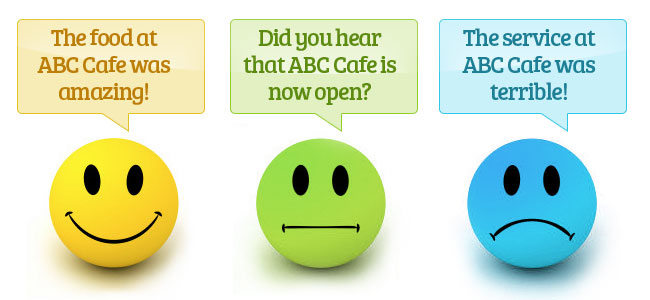
\includegraphics[width=180, height=110]{img1.jpg} 
\end{center}
\end{frame}

\section{Scope of the project}
\begin{frame}[t]
\frametitle{Scope of the project}
\begin{enumerate}
\item Consumers can use sentiment analysis to research products or services before making a purchase \cite{rp9}. Eg: Kindle.
\item Marketers can use this to research public opinion of their company and products, or to analyze customer satisfaction. Eg: Election Polls \cite{rp1}.
\item Organizations can also use this to gather critical feedback about problems in newly released products. Eg: Brand Management (Nike, Adidas).
\end{enumerate}
\end{frame}

\section{Tools used}
\begin{frame}[t]
\frametitle{Tools used}
Tools used are as follows:
\begin{enumerate}

 \item \textbf{\underline{Python}} \cite{python}: It is a widely used general-purpose, high-level programming language.
 \item \textbf{\underline{Natural Language Toolkit (NLTK)}} \cite{nltk}: It is a leading platform for building Python programs to work with human language data. It provides a suite of text processing libraries for classification, tokenization, etc.
 \item \textbf{\underline{LIBSVM}} \cite{libsvm}: A Library for Support Vector Machines.
\end{enumerate}
\begin{center}

\includegraphics[width=150, height=90]{img2.png} 
\end{center}
\end{frame}

\section{Fetching Tweets}
\begin{frame}[t]
\frametitle{Fetching Tweets}
To fetch a tweet:
\begin{enumerate}
\item Create a twitter account if you do not already have one.
\item Go to https://dev.twitter.com/apps and log in with your twitter credentials and "Create New App".
\item Fill out the form and agree to the terms. This generates four keys: \textbf{api key, api secret key, access token key, and access secret key}.
\item Python code: Construct an oauth request, sign the request, and open a twitter request using the credentials above.
\item Python code: With the help of OpenerDirector instance of urllib module fetch the tweets in JSON format.
\item Python code: Tweets in JSON format having lang field as "en" are then processed further. The tweet is in "text" field.
\end{enumerate}
\end{frame}

\section{Preprocessing Tweets}
\begin{frame}[t]
\frametitle{Preprocessing Tweets}
Preprocessing tweets includes:
\begin{enumerate}
\item Getting the tweet from the "text" field of a JSON document.
\item Convert the tweets to lower case.
\item Eliminate all of these URLs via regular expression matching or replace with generic word URL.
\item Eliminate '@username' via regex matching or replace it with generic word AT\_USER.
\item Hashtags can give us some useful information, so it is useful to replace them with the exact same word without the hash. E.g. \#nike replaced with 'nike'.
\item Remove punctuation at the start and ending of the tweets. E.g: 'the day is beautiful!' replaced with 'the day is beautiful'.
\item Remove additional white space.
\end{enumerate}
\end{frame}

\section{Approaches used}
\begin{frame}[t]
\frametitle{Approaches used}
\begin{enumerate}
\item Sentiment Dictionary Approach.
\item Naive Bayes Approach.
\item Support Vector Machines (SVM) Approach.
\end{enumerate}
\end{frame}

\begin{frame}[t]
\frametitle{Sentiment Dictionary Approach: Overview}
\begin{enumerate}
\item A file having 2482 words and their sentiment value (ranging from -5 to 5) is maintained. We call this file Sentiment Dictionary. \cite{sentimentdictionary}
\item A word and its sentiment in the Sentiment Dictionary is seperated by a tab character, i.e., '\textbackslash t'.
\item A very positive word like 'happy' is given a sentiment value of 5.
\item A neutral word like 'aeroplane' is given a sentiment value close to 0.
\item A very negative word like 'hate' is given a sentiment value of -5.
\end{enumerate}
\end{frame}

\begin{frame}[t]
\frametitle{Sentiment Dictionary Approach: Algorithm}
The algorithm for Sentiment Dictionary Approach is as follows:
\begin{enumerate}
 \item Get all the words present in the tweet.
 \item Add the sentiment value of all words while referring to the Sentiment Dictionary. 
 If the word is not present in the Sentiment Dictionary then add 0.
 \item If the cumulative sentiment value is positive then the tweet is positive.
 \item If the cumulative sentiment value is zero then the tweet is neutral.
 \item If the cumulative sentiment value is negative then the tweet is negative.
\end{enumerate}
\end{frame}

\begin{frame}[t]
\frametitle{Sentiment Dictionary Approach: Example}
\begin{table}[h]
\begin{tabular}{|l|l|l|l|}
\hline
Words in tweet  & I & like & cars \\ \hline
Sentiment value & 0 & 2    & 0    \\ \hline
\end{tabular}
\caption{Cumulative sentiment value: 2. Tweet is classified as positive.}
\end{table}

\begin{table}[h]
\begin{tabular}{|l|l|l|l|l|}
\hline
Words in tweet  & My & name & is & Ram \\ \hline
Sentiment value & 0  & 0    & 0  & 0   \\ \hline
\end{tabular}
\caption{Cumulative sentiment value: 0. Tweet is classified as neutral.}
\end{table}

\begin{table}[h]
\begin{tabular}{|l|l|l|l|}
\hline
Words in tweet  & I & hate & cars \\ \hline
Sentiment value & 0 & -3    & 0    \\ \hline
\end{tabular}
\caption{Cumulative sentiment value: -3. Tweet is classified as negative.}
\end{table}
\end{frame}

\begin{frame}[t]
\frametitle{Sentiment Dictionary Approach: Problems}
Problems in Sentiment Dictionary Approach are as follows:
\begin{enumerate}
\item If all the the words of the tweet are not present in the Sentiment Dictionary then the tweet will be judged as neutral which is not necessarily true always.
\item If a tweet has positive and negative words as per the Sentiment Dictionary, then they can very well add upto 0. Thereby, the tweet will be judged as neutral which is not necessarily true always.
\end{enumerate}
\begin{center}

\includegraphics[width=90, height=75]{img3.jpg} 
\end{center}
\end{frame}

\begin{frame}[t]
\frametitle{Sentiment Dictionary Approach: Results}
1000 testing tweets (367 positive, 418 neutral and 215 negative tweets) were tested against 2482 words of the Sentiment Dictionary. The results are tabulated below:\\
\begin{table}[h]
\begin{tabular}{c|c|c|c|}
\cline{2-4}
                                                  & \multicolumn{3}{c|}{Judged as}                                                                                   \\ \cline{2-4} 
\multirow{-2}{*}{}                                & Positive                           & Neutral                              & Negative                             \\ \hline
\multicolumn{1}{|c|}{Positive Testing Tweets (367)} & {\color[HTML]{036400} \textbf{206}} & {\color[HTML]{680100} 152}            & {\color[HTML]{680100} 9}            \\ \hline
\multicolumn{1}{|c|}{Neutral Testing Tweets (418)}  & {\color[HTML]{680100} 33}        & {\color[HTML]{036400} \textbf{358}} & {\color[HTML]{680100} 27}          \\ \hline
\multicolumn{1}{|c|}{Negative Testing Tweets (215)} & {\color[HTML]{680100} 17}        & {\color[HTML]{680100} 59}          & {\color[HTML]{036400} \textbf{139}} \\ \hline
\end{tabular}
\caption{Sentiment Dictionary Approach Analysis.}
Overall Accuracy: 70.3 \%
\par\smallskip
\end{table}
\end{frame}

%%%%%%%%%%%%%%%%%%%%%%%%%%%%%%%%%%%%%%%%%%%%%%%%%%%%%%%%

\begin{frame}[t]
\frametitle{Naive Bayes Approach: Overview \cite{naivebayes1}}
The data that has been successfully ported are as follows:
\begin{enumerate}
 \item The Naive Bayes classifier is perhaps the simplest trained, probabilistic classifier model.
 \item Also known as simple Bayes or independence Bayes.
 \item Naive Bayes classifiers can be trained very efficiently in a supervised learning setting.
 \item An advantage of naive Bayes is that it only requires a small amount of training data to estimate the parameters necessary for classification.
\end{enumerate}
\end{frame}

\begin{frame}[t]
\frametitle{Naive Bayes Approach: Algorithm \cite{naivebayes}}
\begin{enumerate}
\item Preprocess the testing tweets.
\item Remove all the stopwords (this, I, etc.) from the training and testing set.
\item Estimate the probability P(c) of each class c by dividing the number of words in tweets in c by the total number of words in the training data set.
\item Estimate the probability distribution P\((w \mid c\)) for all words w and classes c. This can be done by dividing the number of occurences of w in tweets in c by the total number of words in c.
\item To find the score of a tweet t for class c, calculate: \\
\begin{center}
score(t, c) = P(c) * $\prod\limits_{i=1}^{n}$ P\((w_i \mid c\))
\end{center}
\item To predict the most likely class label, just pick the c with the highest score value.
\end{enumerate}
\end{frame}

\begin{frame}[t]
\frametitle{Naive Bayes Approach: Example}
There are 16905 words (5830, 5320, 5755 words in the positive, neutral and negative respectively) in the training data set.
\begin{table}[h]
\begin{tabular}{|l|l|l|l|l|}
\hline
Words in tweet  & I & like  & cars \\ \hline
Probability(positive) & -  & 8/5830    & 1/5830   \\ \hline
Probability(neutral) & -  & 2/5320  & 3/5320   \\ \hline
Probability(negative) & -  & 1/5755  & 1/5755   \\ \hline
\end{tabular}
\end{table}
\begin{table}[h]
\begin{tabular}{|c|c|}
\hline
Positive score & 5830/16905 * 8/5830 * 1/5830 = \textbf{0.000000081} \\ \hline
Neutral score  & 5320/16905 * 2/5320 * 3/5320 = 0.000000067 \\ \hline
Negative score & 5755/16905 * 1/5755 * 1/5755 = 0.000000010 \\ \hline
\end{tabular}
\\~
\\ Tweet classified as: Positive.
\end{table}
\end{frame}

\begin{frame}[t]
\frametitle{Naive Bayes Approach: Problems}
Problems in Naive Bayes Approach are as follows:
\begin{enumerate}
\item It assumes each feature to be independent of all other features. This is the "naive" assumption seen in the multiplication of P\((w_i \mid c\)) in the definition of score. Thus, for example, if there is a feature 'best' and another 'world's best', then their probabilities would be multiplied as though independent, even though the two are overlapping. 
\item The same issues arise for words that are highly correlated with other words (idioms, phrases, etc.).
\item Training time is high.
\item If there is no occurence of a word in a class and the word is present in the test tweet then after multiplication the score of the tweet will come as 0.
\end{enumerate}
\end{frame}

\begin{frame}[t]
\frametitle{Naive Bayes Approach: Results}
1000 testing tweets (367 positive, 418 neutral and 215 negative tweets) were tested against 1500 tweets \cite{dataset} (500 positive, 500 neutral and 500 negative tweets). The results are tabulated below:\\
\begin{table}[h]
\begin{tabular}{c|c|c|c|}
\cline{2-4}
                                                  & \multicolumn{3}{c|}{Judged as}                                                                                   \\ \cline{2-4} 
\multirow{-2}{*}{}                                & Positive                           & Neutral                              & Negative                             \\ \hline
\multicolumn{1}{|c|}{Positive Testing Tweets (367)} & {\color[HTML]{036400} \textbf{194}} & {\color[HTML]{680100} 89}            & {\color[HTML]{680100} 84}            \\ \hline
\multicolumn{1}{|c|}{Neutral Testing Tweets (418)}  & {\color[HTML]{680100} 24}        & {\color[HTML]{036400} \textbf{347}} & {\color[HTML]{680100} 47}          \\ \hline
\multicolumn{1}{|c|}{Negative Testing Tweets (215)} & {\color[HTML]{680100} 21}        & {\color[HTML]{680100} 53}          & {\color[HTML]{036400} \textbf{141}} \\ \hline
\end{tabular}
\caption{Naive Bayes Approach Analysis.}
Overall Accuracy: 68.2 \%
\par\smallskip
\end{table}
\end{frame}

%%%%%%%%%%%%%%%%%%%%%%%%%%%%%%%%%%%%%%

\begin{frame}[t]
\frametitle{Support Vector Machines Approach: Overview \cite{svm}}
\begin{itemize}
 \item Supervised learning model with associated learning algorithms that analyzes data and is used for classification.
 \item A data point is viewed as a p dimensional vector, and we want to know whether we can separate such points with a (p-1) dimensional hyperplane. 
 \item The best hyperplane is the one that represents the largest separation, or margin, between the two classes.
 \item New examples are then mapped into that same space and predicted to belong to a category based on which side of the gap they fall on.
 \end{itemize}
\end{frame}

\begin{frame}[t]
\frametitle{Support Vector Machines Approach: Overview \cite{svm}}
\begin{center}
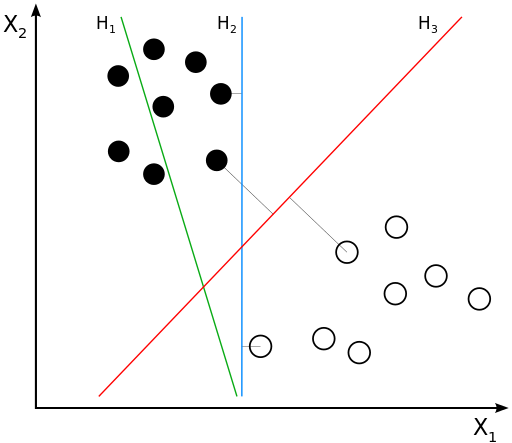
\includegraphics[width=5.5cm, height=5cm]{images/svm1}
\\H1 does not separate the classes. H2 does, but only with a small margin. H3 separates them with the maximum margin.
\end{center}
\end{frame}

\begin{frame}[t]
\frametitle{Support Vector Machines Approach: Overview \cite{svm}}
\begin{itemize}
 \item Given some training data $\mathcal{D}$, a set of n points of the form: 
 \begin{center}
 $\mathcal{D} = \left\{ (\mathbf{x}_i, y_i)\mid\mathbf{x}_i \in \mathbb{R}^p,\, y_i \in \{-1,1\}\right\}_{i=1}^n$
  \end{center}
 \item Any hyperplane can be written as the set of points $\mathbf{x}$ satisfying: 
  \begin{center}$\mathbf{w}\cdot\mathbf{x} - b=0.$ \end{center}
  where $\cdot$ denotes the dot product and ${\mathbf{w}}$ the normal vector to the hyperplane. 
 \item By using geometry, we find the distance between these two hyperplanes is $\tfrac{2}{\|\mathbf{w}\|}$, so we want to minimize $\|\mathbf{w}\|$. 
 \end{itemize}
\end{frame}

\begin{frame}[t]
\frametitle{Support Vector Machines Approach: Overview \cite{svm}}
\begin{center}
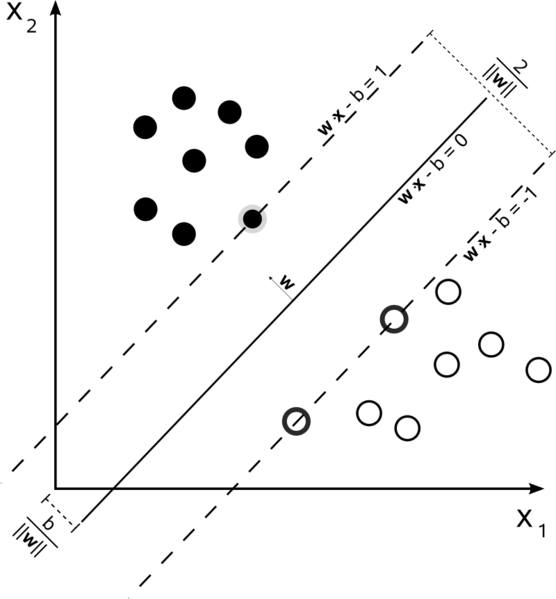
\includegraphics[width=5cm, height=5cm]{images/svm2}
\\Maximum-margin hyperplane and margins for an SVM trained with samples from two classes. Samples on the margin are called the support vectors.
\end{center}
\end{frame}

\begin{frame}[t]
\frametitle{Support Vector Machines Approach: Overview \cite{svm}}
\begin{itemize}
 \item To minimize $\|\mathbf{w}\|$, $\|\mathbf{w}\|^2$ is minimized.
 \  \\
 \  \\
 \item This is a quadratic programming optimization problem:
\begin{center}
$\arg\min_{(\mathbf{w},b)}\|\mathbf{w}\|^2$
\\ subject to $y_i(\mathbf{w}\cdot\mathbf{x_i} - b) \ge 1$ \\ (for any i = 1, \dots, n).
\end{center}
\  \\
\  \\
\item By introducing Lagrange multipliers $\boldsymbol{\alpha}$:

\begin{center}
$\arg\min_{(\mathbf{w},b)} \max_{(\boldsymbol{\alpha}\geq 0)} \left\{ \|\mathbf{w}\|^2 - \sum_{i=1}^{n}{\alpha_i[y_i(\mathbf{w}\cdot \mathbf{x_i} - b)-1]} \right\}$
\end{center}
\  \\
\  \\
\item This problem can now be solved by standard quadratic programming techniques leading to:
\begin{center}
$\mathbf{w} = \sum_{i=1}^n{\alpha_i y_i\mathbf{x_i}}$.\\
\end{center}
\end{itemize}
\end{frame}

\begin{frame}[t]
\frametitle{Support Vector Machines Approach: Algorithm}
Algorithm implemented using LIBSVM is shown below:
\begin{enumerate}
 \item Train the linear multiclass SVM classifier based on training tweet data set \cite{dataset}. 
 Each training tweet is mapped into the hyperplane with help of its feature list.
 \item Preprocess the testing tweets and build a feature list for each tweet.
 \item Map each testing tweet into the hyperplane with help of its feature list to know the class of the tweet.
\end{enumerate}
\end{frame}

\begin{frame}[t]
\frametitle{Support Vector Machines Approach: Problems}
Problems in Support Vector Machines Approach are as follows:
\begin{enumerate}
 \item Parameters of a solved model were difficult to interpret.
 \item Length of feature list is huge.
\end{enumerate}
\end{frame}

\begin{frame}[t]
\frametitle{Support Vector Machines Approach: Results}
1000 testing tweets (367 positive, 418 neutral and 215 negative tweets) were tested against 4550 tweets (2441 positive, 689 neutral and 1720 negative tweets). The results are tabulated below:\\
\begin{table}[h]
\begin{tabular}{c|c|c|c|}
\cline{2-4}
                                                  & \multicolumn{3}{c|}{Judged as}                                                                                   \\ \cline{2-4} 
\multirow{-2}{*}{}                                & Positive                           & Neutral                              & Negative                             \\ \hline
\multicolumn{1}{|c|}{Positive Testing Tweets (367)} & {\color[HTML]{036400} \textbf{272}} & {\color[HTML]{680100} 53}            & {\color[HTML]{680100} 42}            \\ \hline
\multicolumn{1}{|c|}{Neutral Testing Tweets (418)}  & {\color[HTML]{680100} 73}        & {\color[HTML]{036400} \textbf{332}} & {\color[HTML]{680100} 13}          \\ \hline
\multicolumn{1}{|c|}{Negative Testing Tweets (215)} & {\color[HTML]{680100} 23}        & {\color[HTML]{680100} 39}          & {\color[HTML]{036400} \textbf{153}} \\ \hline
\end{tabular}
\caption{Support Vector Machines Approach Analysis.}
Overall Accuracy: 75.7 \%
\par\smallskip
\end{table}
\end{frame}

%%%%%%%%%%%%%%%%%%%%%%%%%%%%%%%%%%%%%%

\section{Future Work}
\begin{frame}[t]
\frametitle{Future Work}
Some of the future work to be done are as follows:
\begin{enumerate}
\item Using maximum entropy classifier and random forest \cite{rp8}.
\item Internationalisation \cite{rp3}: Classify tweets of all languages.
\item Semantics \cite{rp6}: Focusing on the relation between words, phrases, etc. Eg: 'Australia beats India' is positive for Australia and negative for India.
\item Bi-grams and Tri-grams \cite{rp7}: Taking two or three words into consideration at the same time.
\end{enumerate}
\begin{center}

\includegraphics[width=70, height=75]{img4.png} 
\end{center}

\end{frame}

\section{Conclusion}
\begin{frame}
\frametitle{Conclusion}
\begin{itemize}
\item Accuracy of classification depends on the training dataset.
\item Accuracy of classification depends on the method used to classify.
\item Using a novel feature vector of weighted unigrams Support Vector Machines can achieve competitive accuracy in classifying tweet sentiment.
\end{itemize}
\\Following is the summary of the accuracies of all the approaches used:
\begin{table}[h]
\begin{tabular}{|c|c|}
\hline
\textbf{Approach used}  & \textbf{Accuracy} \\ \hline
Sentiment Dictionary    & 70.3 \%          \\ \hline
Naive Bayes             & 68.2 \%          \\ \hline
Support Vector Machines & 75.7 \%           \\ \hline
\end{tabular}
\end{table}
\end{frame}

%---------------------------------------------------------------------------------------
%     Final Slide - References
%--------------------------------------------------------------------------------------
\section{References}
\frametitle{References}
\begin{frame}[allowframebreaks]{References}
\bibliographystyle{ieeetr}
\bibliography{biblio}
\end{frame}

\section*{Thank You}
\begin{frame}[t]
\frametitle{Thank You!}
\begin{center}

\includegraphics[width=7cm, height=5cm]{images/thankyou} 
\end{center}
\end{frame}
\end{document}